\documentclass{article}
\usepackage[margin=1in]{geometry}
\usepackage{amsmath, amsthm, amssymb, fancyhdr, tikz, circuitikz, graphicx}
\usepackage{centernot, xcolor, hhline, multirow, listings, dashrule}
\usepackage{blkarray, booktabs, bigstrut, etoolbox, extarrows}
\usepackage[normalem]{ulem}
\usepackage{bookmark}
\usetikzlibrary{math}
\usetikzlibrary{fit}

\pagestyle{fancy}

\usepackage{hyperref}
\hypersetup{
  colorlinks=true,
  linkcolor=black,
  filecolor=magenta,
  urlcolor=cyan,
}
%formatting
\newcommand{\bld}{\textbf}
\newcommand{\itl}{\textit}
\newcommand{\uln}{\underline}

%math word symbols
\newcommand{\bb}{\mathbb}
\DeclareMathOperator{\tif}{~\text{if}~}
\DeclareMathOperator{\tand}{~\text{and}~}
\DeclareMathOperator{\tbut}{~\text{but}~}
\DeclareMathOperator{\tor}{~\text{or}~}
\DeclareMathOperator{\tsuchthat}{~\text{such that}~}
\DeclareMathOperator{\tsince}{~\text{since}~}
\DeclareMathOperator{\twhen}{~\text{when}~}
\DeclareMathOperator{\twhere}{~\text{where}~}
\DeclareMathOperator{\tfor}{~\text{for}~}
\DeclareMathOperator{\tthen}{~\text{then}~}
\DeclareMathOperator{\tto}{~\text{to}~}
\DeclareMathOperator{\tin}{~\text{in}~}

%display shortcut
\DeclareMathOperator{\dstyle}{\displaystyle}
\DeclareMathOperator{\sstyle}{\scriptstyle}

%linear algebra
\DeclareMathOperator{\id}{\bld{id}}
\DeclareMathOperator{\vecspan}{\text{span}}
\DeclareMathOperator{\adj}{\text{adj}}

%discrete math - integer properties
\DeclareMathOperator{\tdiv}{\text{div}}
\DeclareMathOperator{\tmod}{\text{mod}}
\DeclareMathOperator{\lcm}{\text{lcm}}

%augmented matrix environment
\newenvironment{apmatrix}[2]{%
  \left(\begin{array}{@{~}*{#1}{c}|@{~}*{#2}{c}}
    }{
  \end{array}\right)
}
\newenvironment{abmatrix}[2]{%
  \left[\begin{array}{@{~}*{#1}{c}|@{~}*{#2}{c}}
      }{
    \end{array}\right]
}

\newenvironment{determinant}[1]{
  \left\lvert
  \begin{array}{@{~}*{#1}{c}}
    }{
  \end{array}
  \right\rvert
}

%lists
\newcommand{\bitem}[1]{\item[\bld{#1.}]}
\newcommand{\bbitem}[2]{\item[\bld{#1.}] \bld{#2}}
\newcommand{\biitem}[2]{\item[\bld{#1.}] \itl{#2}}
\newcommand{\iitem}[1]{\item[\itl{#1.}]}
\newcommand{\iiitem}[2]{\item[\itl{#1.}] \bld{#2}}
\newcommand{\btitem}[2]{\item[\bld{#1.}] \texttt{#2}}

%homework
\newcommand{\question}[2]{\noindent {\large\bld{#1}} #2 \qline}
\newcommand{\qitem}[3]{\item[\bld{#1.}] #2 \qdash \\ #3 \qdash}

\newcommand{\qline}{~\newline\noindent\textcolor[RGB]{200,200,200}{\rule[0.5ex]{\linewidth}{0.2pt}}}
\newcommand{\qdash}{~\newline\noindent\textcolor[RGB]{200,200,200}{\hdashrule[0.5ex]{\linewidth}{0.2pt}{2pt}}}

\begin{document}

%use for sets with non-alphanumeric characters
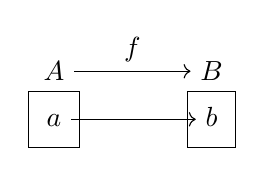
\begin{tikzpicture}
    \foreach[count=\i] \set/\elements in {$A$/{$a$}, $B$/{$b$}} { %domain and co-domain
    \begin{scope}[local bounding box=\set, x=2cm, y=0.5cm]
        \foreach[count=\j] \element in \elements {
            \node[minimum width=1em,anchor=base,text height=1.4ex,text depth=0.25ex]
            (\i-\j) at (\i,-\j) {\element};
        }
    \end{scope}
    \node[draw, fit=(\set), label={[name=\i]above:\set}] {};
    }
    \foreach \domain/\target in {1/1} { %function pairs, uses indices
            \draw[->] (1-\domain) -- (2-\target);
        }
    \draw[->] (1) -- node[above]{$f$}(2); %function name
\end{tikzpicture}


%use for sets for only alphanumeric characters
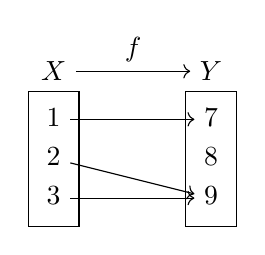
\begin{tikzpicture}
    \foreach[count=\i] \set/\elements in {X/{1,2,3}, Y/{7,8,9}} { %domain and co-domain
    \begin{scope}[local bounding box=\set, x=2cm, y=0.5cm]
        \foreach[count=\j] \element in \elements {
            \node[minimum width=1em,anchor=base,text height=1.4ex,text depth=0.25ex]
            (\i-\element) at (\i,-\j) {$\element$};
        }
    \end{scope}
    \node[draw, fit=(\set), label={[name=\i]above:$\set$}] {};
    }
    \foreach \domain/\target in {1/7,2/9,3/9} { %function pairs, uses indices
            \draw[->] (1-\domain) -- (2-\target);
        }
    \draw[->] (1) -- node[above]{$f$}(2); %function name
\end{tikzpicture}


%use for digraphs for center
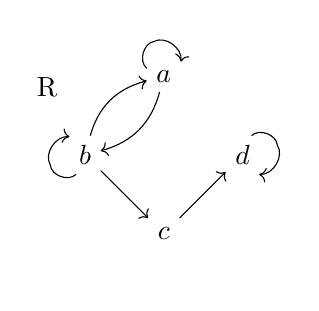
\begin{tikzpicture}
    %VARIABLES
    \pgfmathsetmacro{\gsize}{1};
    \pgfmathsetmacro{\gnum}{4};

    \foreach[count=\i] \element in {a,b,c,d} { %domain
            \node (\element) at (\i * 360 / \gnum:\gsize) {$\element$};
            \node (\element-) at (\i * 360 / \gnum:\gsize + 0.5) {};
        }
    \foreach \j/\l in {b/c, c/d} { %a to b
            \draw[->] (\j) -- (\l);
        }
    \foreach \j/\l in {a/b} { %a to b AND b to a
            \draw[->] (\j) to[bend left=20 / \gsize + 10] (\l);
            \draw[->] (\l) to[bend left=20 / \gsize + 10] (\j);
        }
    \foreach \j in {a,b,d} { %a to a
            \draw[->] (\j) to[bend left=65] (\j-)
            to[bend left=65] (\j);
        }
    \node[anchor=east] (name) at (145:\gsize+.5) {R}; %relation name
\end{tikzpicture}

%use for undirected graphs for center
\begin{tikzpicture}
    %VARIABLES
    \pgfmathsetmacro{\gsize}{1};
    \pgfmathsetmacro{\gnum}{4};

    \foreach[count=\i] \element in {a,b,c,d} { %domain
            \node (\element) at (\i * 360 / \gnum:\gsize) {$\element$};
            \node (\element-) at (\i * 360 / \gnum:\gsize + 0.5) {};
        }
    \foreach \j/\l in {b/c, c/d} { %a to b
            \draw (\j) -- (\l);
        }
    \foreach \j in {a,b,d} { %a to a
            \draw (\j) to[bend left=65] (\j-)
            to[bend left=65] (\j);
        }
    \node[anchor=east] (name) at (145:\gsize+.5) {Graph}; %relation name
\end{tikzpicture}

%use for digraphs for center WITH PARALLEL EDGES
\begin{tikzpicture}
    %VARIABLES
    \pgfmathsetmacro{\gsize}{1};
    \pgfmathsetmacro{\gnum}{4};

    \foreach[count=\i] \element in {a,b,c,d} { %domain
            \node (\element) at (\i * 360 / \gnum:\gsize) {$\element$};
            \node (\element-) at (\i * 360 / \gnum:\gsize + 0.5) {};
        }
    \foreach \j/\l in {a/c,b/d,c/d} { %a to b
            \draw (\j) -- (\l);
        }
    \foreach \j/\l in {a/b} { %a to b TWICE (parallel edges)
            \draw (\j) to[bend left=20 / \gsize + 10] (\l);
            \draw (\l) to[bend left=20 / \gsize + 10] (\j);
        }
    \foreach \j in {c} { %a to a
            \draw (\j) to[bend left=65] (\j-)
            to[bend left=65] (\j);
        }
    \node[anchor=east] (name) at (145:\gsize+.5) {A graph with parallel edges and a self-loop}; %relation name
\end{tikzpicture}


%use for Hasse Diagrams
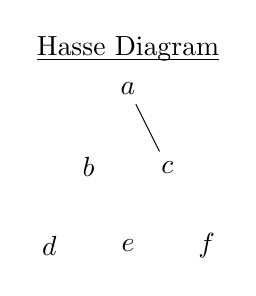
\begin{tikzpicture}
    %VARIABLES
    \pgfmathsetmacro{\gsize}{1};
    \pgfmathsetmacro{\gnum}{4};

    \foreach \rank/\elements/\size in {1/{a}/1, 2/{b,c}/2, 3/{d,e,f}/3} {
    \foreach[count = \i] \element in \elements {\node (\element) at (\i - \size / 2, -\rank) {$\element$};}
    }
    \foreach \j/\l in {a/c} {\draw (\j) -- (\l);}
    \node (name) at (0.5,-0.5) {\underbar{Hasse Diagram}}; %name
\end{tikzpicture}

%turing machine tape
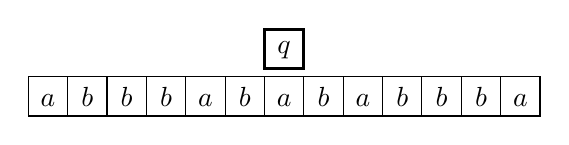
\begin{tikzpicture}
    \pgfmathsetmacro{\x}{0.5};
    \pgfmathsetmacro{\y}{0.5};
    \pgfmathsetmacro{\vset}{0};
    \pgfmathsetmacro{\qset}{7};

    \foreach[count=\i] \element in {a,b,b,b,a,b,a,b,a,b,b,b,a} {
            \draw (\i * \x,0) rectangle ++(\x,\y);
            \node[anchor=south] (\element) at (\i*\x + \x * 0.5, \vset) {$\element$};
        }
    \draw[very thick] (\qset*\x, \y + 0.1) rectangle ++(\x,\y);
    \node[anchor=south] (q) at (\qset*\x + \x*0.5, \y + 0.1) {$q$};
\end{tikzpicture}


\end{document}